\chapter{Avaliação e Resultados}
Neste capítulo serão mostradas uma avaliação heurística, uma avaliação de relevância da aplicação, uma pesquisa de satisfação dos usuários, sugestões enviadas por usuários e estatísticas de uso da aplicação. Todos esses recursos foram utilizados para estimar a qualidade do software MeForma2.

Determinar a qualidade de um software é uma atividade complexa e imprecisa. Em seu trabalho sobre Visões de Qualidade, \cite{garvin} analisa a qualidade sob a perspectiva de diversas áreas do conhecimento, como filosofia, economia e marketing. Ele afirma que ``a qualidade é um conceito complexo que possui muitas faces''. \cite{garvin} considera que a qualidade pode ser descrita sob cinco perspectivas: 
\begin{itemize}
    \item A visão transcendental - que vê qualidade como algo que pode ser reconhecido, mas não definido.
    \item A visão do usuário - que vê qualidade como adequação para um propósito.
    \item A visão do fabricante - que considera a qualidade como conformidade com a especificação.
    \item A visão do produto - vê a qualidade como ligada às características inerentes do produto.
    \item A visão baseada em valor - considera a qualidade como dependente do valor que um cliente está disposto a pagar por ela.
\end{itemize}

Neste trabalho optou-se por avaliar a qualidade do software principalmente sob a perspectiva do usuário. Associou-se a qualidade do software em questão à reação dos usuários ao mesmo. Entendeu-se que se os usuários classificam o software como adequado para o fim proposto, consideram-se satisfeitos com os recursos que o software oferece e estão dispostos a indicá-lo a outras pessoas, então esse é um software de qualidade.

\section{Avaliação Heurística}

A Avaliação Heurística é um método de avaliação de usabilidade de software proposto por \cite{nielsen}. O método permite ao avaliador examinar uma solução para tentar antever as possíveis consequências de certas decisões de design. Esse método de avaliação é categorizado como método de avaliação por inspeção e não envolve os usuários.

Para realizar a avaliação, utilizou-se um conjunto de diretrizes de usabilidade, definidas por Nielsen, chamadas de heurísticas de usabilidade. Uma heurística é uma regra que funciona na prática, mas não exige uma explicação teórica. Foram enumeradas 10 heurísticas:

\begin{itemize}
    \item H1: Visibilidade do status do sistema - O sistema deve sempre manter os usuários informados sobre o que está acontecendo através de \textit{feedback}\footnote{resposta rápida e apropriada} rápido e apropriado.
    \item H2: Correspondência entre o sistema e o mundo real - O sistema deve falar a linguagem do usuário, 0,com palavras, frases e conceitos familiares ao usuário. Ele deve seguir convenções do mundo real, fazendo informações aparecem em uma ordem lógica e natural. 
    \item H3: Controle e liberdade para o usuário - Muitas vezes os usuários podem realizar ações por engano. A aplicação deve permitir que os usuários desfaçam e refaçam suas ações.
    \item H4: Consistência e padronização - O sistema deve seguir as convenções existentes, utilizando sempre as mesmas palavras e ícones para as mesmas ações.
    \item H5: Prevenção de Erros - Um sistema que evite que erros ocorram é ainda melhor que um sistema com boas mensagens de erro.
    \item H6: Reconhecimento ao invés de memorização - O usuário não deve ter que lembrar de informações de outras partes do sistema. Instruções de uso do sistema devem estar sempre visíveis ou serem facilmente encontradas.
    \item H7: Flexibilidade e eficiência no uso - A utilização do sistema deve ser agilizada pelo uso de atalhos.
    \item H8: Design estético e minimalista - O sistema não deve exibir informações desnecessárias, pois elas irão competir com as necessárias.
    \item H9: Ajuda para reconhecer, diagnosticar e se recuperar de erros - Mensagens de erro devem ser claras, indicar o problema e sugerir uma solução.
    \item H10: Ajuda e documentação - O ideal é que o sistema não precise de documentação para ser usado. Pode-se incluir diálogos de ajuda e/ou de uma documentação sucinta.
\end{itemize}

As infrações encontradas foram julgadas a partir da classificação de severidade explicada na Tabela~\ref{severidade}. Esse modelo de classificação foi proposto por \cite{nielsen}.

\begin{table}[H]
\caption{Classificação de severidade de problemas de usabilidade.}
\label{severidade}
\begin{tabular}{ |c|c| } 
 \hline
 Severidade & Explicação \\
 \hline
 0 & Não é encarado como um problema de usabilidade. \\
 \hline
 1 & Problema estético - a ser corrigido apenas se houver tempo disponível. \\
 \hline
 2 &  Problema pequeno - baixa prioridade para sua correção. \\
 \hline
 3 & Problema grande - alta prioridade para sua correção. \\
 \hline
 4 &  Problema catastrófico - é extremamente necessário corrigir. \\
 \hline
\end{tabular}
\end{table}

Para guiar a avaliação, foram selecionados oito cenários de uso do sistema que contemplam as principais telas:

\begin{enumerate}
    \item Como usuário, gostaria de me cadastrar no sistema;
    \item Como usuário, gostaria de selecionar as disciplinas que já cursei;
    \item Como usuário, gostaria de visualizar os pré-requisitos de uma disciplina;
    \item Como usuário, gostaria de cadastrar uma carga horária;
    \item Como usuário, gostaria de cadastrar um semestre;
    \item Como usuário, gostaria de contabilizar minhas faltas em uma disciplina;
    \item Como usuário, gostaria de importar dados do SIAC;
    \item Como usuário, gostaria de visualizar minha completude de curso.
\end{enumerate}

A Tabela~\ref{avaliacaoheuristica} lista e classifica as infrações encontradas no MeForma2 pelo método de avaliação heurística. Nenhuma infração foi classificada com Severidade 4, ou seja, não houveram problemas catastróficos durante a análise, além disso, os demais problemas não exigem mudanças nas regras de negócio da aplicação, pois tratam-se apenas de correções visuais e adição de textos. 

O resultado da avaliação indica que o sistema possui uma interface bem resolvida e intuitiva. O que significa dizer que os usuários terão pouca ou nenhuma dificuldade em utilizar a interface.

\begin{table}[H]
\begin{center}
\caption{Infrações encontradas no MeForma2 pela avaliação heurística.}
\begin{tabular}{ |p{3cm}|c|c|c|p{5.5cm}| }
\hline
 \textbf{Problema} & \textbf{Cenário} & \textbf{Heurísticas} & \textbf{Severidade} & \textbf{Explicação} \\ 
 \hline
 Confirmação de e-mail e senha & 1 & H5 & 3 & O cadastro não exige confirmação de e-mail ou senha, caso o usuário insira dados inválidos, ele pode não conseguir utilizar o sistema posteriormente \\
 \hline
 Estilo dos campos do formulário & 1 & H7 & 1 & Os campos do formulário são diferentes dos utilizados pelo \textit{Android}, o que pode causar confusão ao usuários da versão mobile. \\
 \hline
 Múltiplas ações ao clicar em disciplina & 2 & H5 & 3 & Existem duas ações ao clicar nos cartões das disciplinas. Elas se diferenciam pelo tempo de clique. Isso pode causar confusão e impedir a descoberta de funcionalidades. \\
 \hline
 Legenda na identificação de pré-requisitos & 3 & H6 & 1 & Não existe legenda para indicar qual a cor que representa um pré-requisito e qual a cor que representa uma dependência, mas foi considerado um problema pequeno, pois o usuário pode visualizar a organização temporal das disciplinas. \\
 \hline
 Mensagem de confirmação de alteração de Carga Horária & 4 & H1 & 2 & Não existem mensagens de sucesso após ações de criar, editar ou excluir uma carga horária, contudo, o usuário pode identificar a mudança na lista imediatamente. \\
 \hline
 Falta de informação ao importar dados do SIAC & 7 & H10 & 2 & O sistema não deixa claro quais dados serão importados do SIAC, podendo deixar o usuário confuso sobre o correto funcionamento da funcionalidade. \\
 \hline
\end{tabular}
\end{center}
\label{avaliacaoheuristica}

\end{table}

\section{Avaliação de Relevância da Aplicação}

A Avaliação de Relevância é uma pesquisa realizada com os usuários do MeForma2, grupo composto por estudantes de graduação da Universidade Federal da Bahia, onde a opinião dos usuários determina a relevância da aplicação. A pesquisa foi realizada de modo anônimo.

A avaliação levou em consideração 3 fatores para determinar a relevância do MeForma2 que combinam com o objetivo da aplicação:
\begin{itemize}
    \item É uma ferramenta que ajuda o estudante a organizar sua vida acadêmica;
    \item É uma ferramenta que ajuda o estudante a entender o que é preciso para alcançar a formatura;
    \item É uma ferramenta que ajuda o estudante a ser responsável com o curso;
\end{itemize}

A pesquisa obteve 62 respostas em 13 dias e o resultado apontou o MeForma2 como uma ferramenta relevante para os cursos de graduação da UFBA. Cada critério foi avaliado com notas de 1 a 5, onde 1 significa que o MeForma2 é totalmente irrelevante para aquele quesito e 5 representa que o MeForma2 é muito relevante para aquele quesito.

As Figuras~\ref{organize}, \ref{graduate} e \ref{responsability} exibem os resultados da pesquisa de relevância da aplicação. Os resultados indicam que o MeForma2 está ajudando os estudantes que participaram da avaliação a se organizarem e a compreenderem melhor sua vida acadêmica, além de alertá-los sobre a responsabilidade que eles tem que ter com o próprio curso.

\begin{figure}[H]
	   \centering
	   		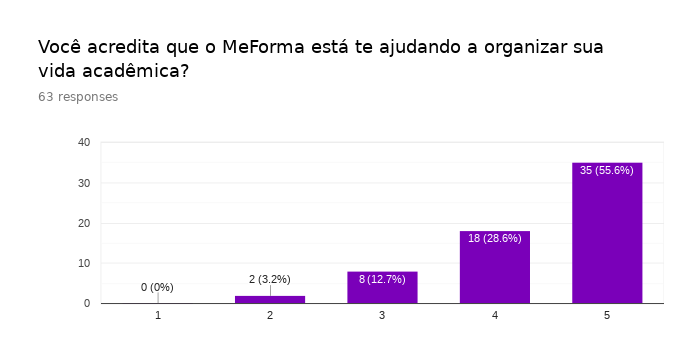
\includegraphics[scale=0.65]{pics/c5/0-organize.png}
	   \caption{Avaliação sobre ajuda com organização de vida acadêmica}
	   \label{organize}
\end{figure}
\begin{figure}[H]
	   \centering
	   		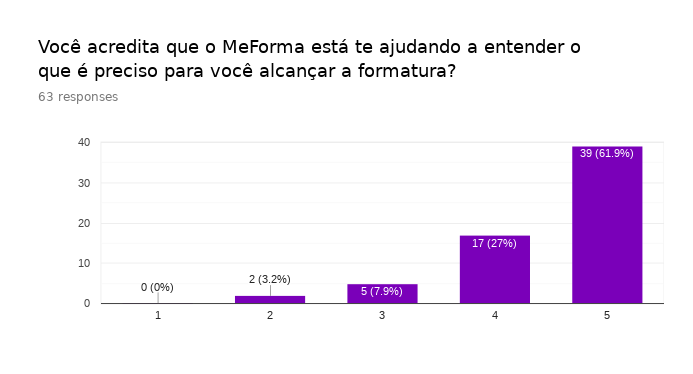
\includegraphics[scale=0.65]{pics/c5/1-graduate.png}
	   \caption{Avaliação sobre entendimento de pré-requisitos para formatura.}
	   \label{graduate}
\end{figure}
\begin{figure}[H]
	   \centering
	   		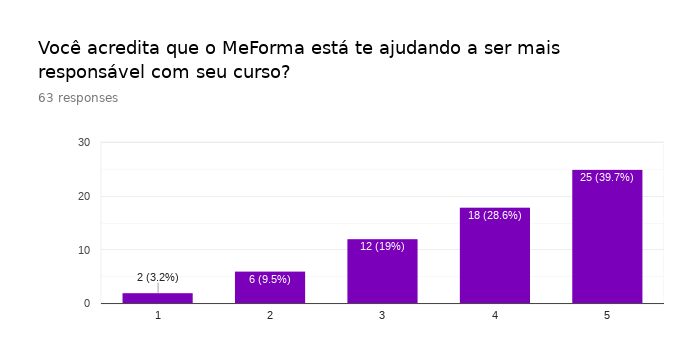
\includegraphics[scale=0.65]{pics/c5/2-responsability.png}
	   \caption{Avaliação sobre responsabilidade com o curso.}
	   \label{responsability}
\end{figure}

\section{Pesquisa de Satisfação}

Esta pesquisa teve a intenção de avaliar dois fatores considerados como fundamentais para o crescimento do MeForma2: o quanto os usuários estavam satisfeitos com o sistema e o quanto eles estavam dispostos a indicar o sistema a outras pessoas. Esses quesitos foram apresentados aos entrevistados como duas perguntas, as quais poderiam ser respondidas com notas de 1 a 5:
\begin{itemize}
    \item Qual o seu nível de satisfação com o MeForma?
    \item Você indicaria o MeForma a um amigo ou colega?
\end{itemize}

A decisão de realizar uma pesquisa de satisfação e os quesitos de avaliação escolhidos tiveram como inspiração as pesquisas de satisfação de cliente realizadas na área de marketing. Segundo Lobos \cite{lobos} "a melhor propaganda é um cliente satisfeito" e "clientes satisfeitos tornam-se apóstolos". Entendeu-se que usuários satisfeitos permanecem utilizando a aplicação e que usuários dispostos a indicar a aplicação atraem novos usuários. 

Os usuários que responderam a pesquisa foram classificados em 3 categorias de acordo com a pergunta "Você indicaria o MeForma a um amigo ou colega?":

\begin{itemize}
    \item Detratores - Usuários que deram nota menor que 3. São pessoas insatisfeitas que podem impedir o crescimento da aplicação através do boca-a-boca negativo.
    \item Neutros - Usuários que deram nota 3 e 4. São clientes satisfeitos, mas que possuem queixas importantes sobre a aplicação. São considerados como vulneráveis a ofertas da concorrência.
    \item Promotores - Usuários que deram nota 5. São clientes leais que vão continuar utilizando a aplicação e a indicarão para outras pessoas.
\end{itemize}

Considerou-se que usuários que demonstraram existir a possibilidade de não indicar o MeForma2 para outras pessoas possuem alguma queixa sobre a aplicação.

\begin{figure}[H]
	   \centering
	   		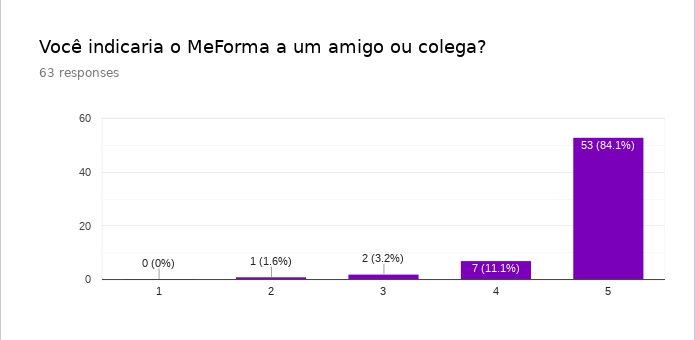
\includegraphics[scale=0.65]{pics/c5/3-share.png}
	   \caption{Disposição dos usuários em indicar o MeForma a outras pessoas.}
	   \label{nps}
\end{figure}

O Figura \ref{nps} mostra a reação dos usuários à pergunta sobre indicar o sistema a outra pessoa. Os resultados indicam que 84,1\% dos entrevistados são Promotores, 1,6\% são Detratores e 14,3\% (3,2\% + 11,1\%) são Neutros. Esse resultado indica que o MeForma2 tem grandes chances de se tornar popular através de divulgação informal proveniente dos próprios usuários, mesmo que alguns deles tenham reclamações a fazer.

\section{Estatísticas de uso da aplicação}

Um diferencial importante trazido pelo MeForma2 foi a publicação de uma plataforma WEB. Muitos usuários da primeira versão do MeForma solicitaram uma versão WEB e, pela característica da aplicação, de ser um serviço de consulta de dados, os usuários se mostravam resistentes a instalar o aplicativo em seus dispositivos.

A divulgação da versão WEB fez com que, não só o número de usuários aumentasse rapidamente, mas também fez com que os acessos ao sistema aumentassem.

Os dados que serão apresentados nesta seção foram computados entre os dias 28 de Outubro de 2018 (Data de lançamento do MeForma2) e 16 de Novembro de 2018, um total de 20 dias.

A Figura \ref{installs} mostra o número de instalações do aplicativo para Android em função do tempo. A linha vertical marca o dia de lançamento do MeForma2. A imagem mostra um crescimento no número de usuários do aplicativo, que saltou de 104 para 141 usuários. A linha tracejada corresponde ao mês anterior, possibilitando visualizar uma queda no número de usuários entre setembro e outubro, e o crescimento entre outubro e novembro.   

\begin{figure}[H]
	   \centering
	   		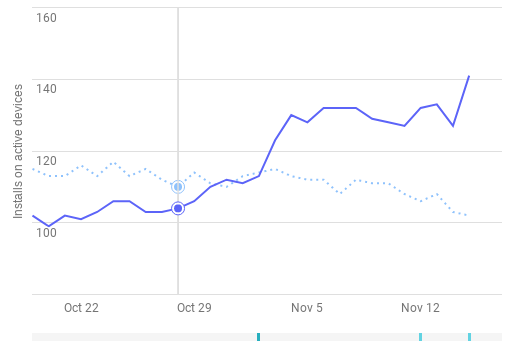
\includegraphics[scale=0.85]{pics/c5/5-installs.png}
	   \caption{Instalações do MeForma para Android.}
	   \label{installs}
\end{figure}

A Figura \ref{web} mostra o número de usuários ativos da versão WEB do MeForma2 em função do tempo. A imagem mostra que a versão WEB teve um número muito maior de usuários, 479 contra 141 do aplicativo. Isso demonstra a preferência do público do MeForma2 pela versão WEB, informação reforçada pelo fato de que na versão web existe o link de download do aplicativo, e as pessoas dão preferência por permanecer na versão web.

\begin{figure}[H]
	   \centering
	   		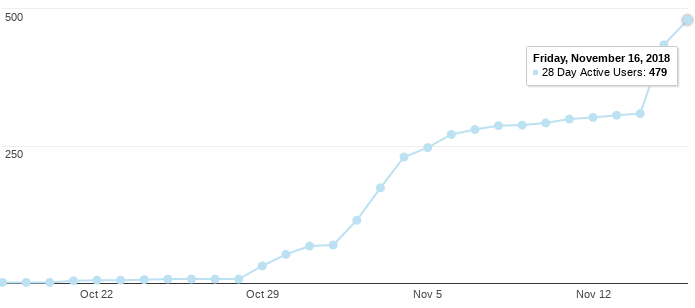
\includegraphics[scale=0.65]{pics/c5/6-active.png}
	   \caption{Utilização do MeForma para WEB}
	   \label{web}
\end{figure}

A Figura \ref{sessions} mostra os dispositivos pelos quais os usuários acessaram a versão WEB do MeForma2.

\begin{figure}[H]
	   \centering
	   		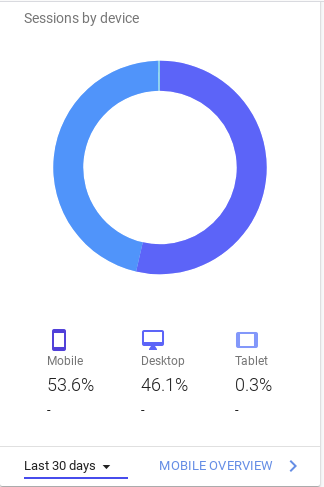
\includegraphics[scale=0.65]{pics/c5/4-sessions.png}
	   \caption{Distribuição do MeForma2 WEB entre os dispositivos.}
	   \label{sessions}
\end{figure}

Uma outra contribuição interessante da versão WEB foi a inclusão de usuários de plataformas mobile diferentes do Android, uma vez que o aplicativo mobile só está disponível para Android. A Figura \ref{mobiles} mostra que o MeForma WEB foi utilizados por usuários do IOS e do Windows, sendo que os usuários do IOS correspondem a 25\% dos usuários da versão WEB em dispositivos móveis.

\begin{figure}[H]
	   \centering
	   		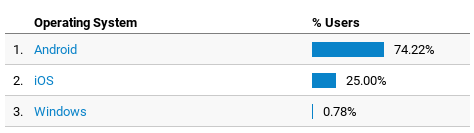
\includegraphics[scale=0.75]{pics/c5/7-mobiles.png}
	   \caption{Distribuição dos usuários mobile por dispositivo.}
	   \label{mobiles}
\end{figure}

A Figura \ref{topcourses} mostra a lista dos 10 cursos que mais utilizam o MeForma. Dando destaque para a porcentagem de usuários dos cursos de Ciência da Computação e Sistemas de Informação que são os cursos que mais se interceptam com o ciclo social do desenvolvedor, e que por causa disso recebem mais informações sobre a aplicação. Levando à intuição de que para se tornar popular entre todos os estudantes da UFBA, a aplicação precisa de um trabalho de divulgação ativo. Até então, toda a divulgação foi feita por Facebook e E-mail.

\begin{figure}[H]
	   \centering
	   		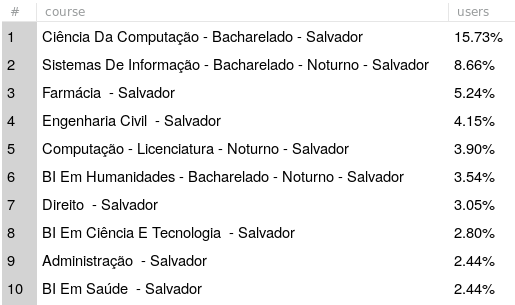
\includegraphics[scale=0.75]{pics/c5/8-topcourses.png}
	   \caption{10 cursos que mais utilizam o MeForma.}
	   \label{topcourses}
\end{figure}

Os dados apresentados até aqui são bastante úteis para entender o público do MeForma2.

\section{Sugestões dos Usuários}

As pesquisas realizadas com os usuários continham um campo para envio de comentários. No total foram enviados 23 comentários, dos quais 14 continham mensagens positivas de parabenização ou elogio.

\say{O aplicativo está muito bom, está atendendo minhas necessidades de forma excelente. Parabéns}

\say{Ótima aplicação, não consigo me imaginar sem ela. Totalmente excepcional!}

\say{Me ajudou bastante pra saber quanto eu faltava de carga horária.}

\say{O que eu mais esperava era a versão web. Amém!}

Dentre os 23 comentários, 7 continham alguma sugestão de melhoria para a aplicação.
 
\say{Acho que na parte de faltas em cada matéria, poderia ter uma opção de ordenar pela matéria com maior número de faltas.}
 
\say{Como venho de transferência interna, no início, tomei um pequeno susto ao perceber que o MeForma não importou automaticamente os dados de disciplinas que eu fiz aproveitamento de estudos (classificados no siac como "Dispensado"), seria bacana se isso já fosse feito direto na importação de dados de alguma forma.}
 
\say{Talvez mudar a cor do botão "importar do siac" para ficar mais visível}
 
 \say{Ao clicar para recuperar senha, sugiro mais instruções no e-mail.}
 
2 dos usuários demonstraram confusão em seus comentários.
 
\say{Não entendi porque em currículo só existem 3 opções e só vai até 2013.2}
 
\say{Não entendi o menu "CH", para mim só aparece que não tenho nada, mesmo eu tendo a carga horária optativa.}

Não houveram comentários negativos, o que indica que a plataforma, mesmo não agradando totalmente 100\% dos usuários, não desagrada ninguém ao ponto de a pessoa fazer uma reclamação direta.

\section{Interesse Externo}

Estudantes de outras instituições ao ter algum contato com o MeForma enviaram mensagens demonstrando interesse e questionando se era possível utilizar em sua instituição. A Tabela \ref{interesse} mostra as instituições representadas e a quantidade de contatos estabelecidos.

\begin{table}[H]
\begin{center}
\begin{tabular}{ |p{10cm}|p{2cm}| }
\hline
Instituição & Contatos \\
\hline
UFpel - Universidade Federal de Pelotas  & 3 \\
\hline
UFRB & 3 \\
\hline
Universidade Estácio de Sá & 2 \\
\hline
Universidade Federal de São João Del Rei & 2 \\
\hline
Anhanguera & 1 \\
\hline
Colégio estadual professor jose Accioli & 1 \\
\hline
Estacio fic do Ceará & 1 \\
\hline
Faculdade jk de Santa maria & 1 \\
\hline
Faculdade Nobre & 1 \\
\hline
FTC & 1 \\
\hline
Ifba & 1 \\
\hline
IFSC & 1 \\
\hline
UCS & 1 \\
\hline
UFES & 1 \\
\hline
UFPB & 1 \\
\hline
UFPE & 1 \\
\hline
UFS & 1 \\
\hline
UNIFACS & 1 \\
\hline
UNIMEP - Universidade Metodista de Piracicaba  & 1 \\
\hline
Universidade Castelo Branco & 1 \\
\hline
Universidade estadual do sudoeste da Bahia  & 1 \\
\hline
Universidade Federal de Roraima & 1 \\
\hline
Universidade Federal do oeste da bahia  & 1 \\
\hline
Urgs & 1 \\
\hline
\end{tabular}
\end{center}
\label{interesse}
\caption{Instituições de ensino representadas na demonstração de interesse pelo MeForma}
\end{table}

\section{Otimização do aplicativo para Android}

Um dos parâmetros para determinar a qualidade de um aplicativo para Android é o tempo de início do aplicativo. De acordo com a documentação do Android, os usuários esperam que os aplicativos sejam responsivos e rápidos para carregar. Um aplicativo com um tempo de início lento não atende a essa expectativa e pode ser decepcionante para os usuários. Esse tipo de experiência insatisfatória pode fazer com que um usuário avalie mal um aplicativo na Play Store ou até mesmo abandone o aplicativo completamente.

O MeForma teve duas grandes versões do aplicativo lançadas, e sete versões de correção e melhoria de funcionalidades. A Figura~\ref{startuptime} mostra o gráfico que compara o desempenho com relação ao tempo de início das versões do aplicativo MeForma. Os valores utilizados para construir o gráfico da Figura~\ref{startuptime} foram obtidos através de uma média aritimética entre 5 cronometragens de inicialização feitas para cada versão. A Tabela~\ref{startuptime2} mostra os tempos em segundos obtidos em cada teste e a média obtida.

\begin{figure}[H]
	   \centering
	   		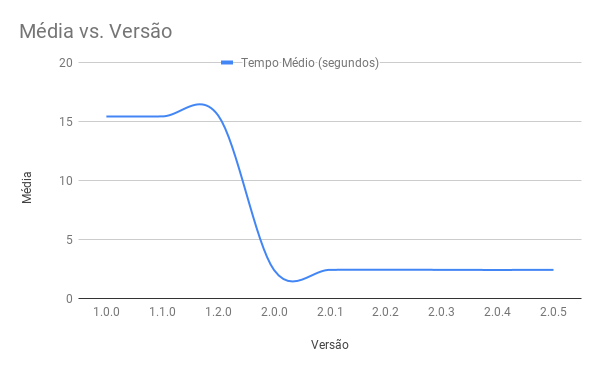
\includegraphics[scale=0.65]{pics/c5/9-startuptime.png}
	   \caption{Tempo médio de inicialização do MeForma por versão e subversão.}
	   \label{startuptime}
\end{figure}

\begin{table}[H]
\begin{center}
\caption{Tempo de inicialização do MeForma por versão.}
\begin{tabular}{ |c|c|c|c|c|c|c| }
\hline
 \textbf{Versão} & \textbf{Teste 1} & \textbf{Teste 2} & \textbf{Teste 3} & \textbf{Teste 4} & \textbf{Teste 5} & \textbf{Média (s)} \\ 
 \hline
 \textbf{1.0.0} & {15.78} &	{15.41} &	{15.29} &	{15.42} &	{15.8} &	{15.42} \\
 \hline 
 \textbf{1.1.0} & {15.43} &	{15.35} &	{15.55} &	{15.29} &	{15.43} &	{15.43} \\
 \hline 
 \textbf{1.2.0} & {15.38} &	{15.55} &	{15.51} &	{15.48} &	{15.7} &	{15.51} \\
 \hline 
 \textbf{2.0.0} & {2.3} &	{2.43} &	{2.41} &	{2.43} &	{2.36} &	{2.41} \\
 \hline 
 \textbf{2.0.1} & {2.54} &	{2.3} &	{2.4} &	{2.43} &	{2.44} &	{2.43} \\
 \hline 
 \textbf{2.0.2} & {2.49} &	{2.22} &	{2.44} &	{2.2} &	{2.5} &	{2.44} \\
 \hline 
 \textbf{2.0.3} & {2.38} &	{2.5} &	{2.45} &	{2.43} &	{2.38} &	{2.43} \\
 \hline 
 \textbf{2.0.4} & {2.44} &	{2.42} &	{2.46} &	{2.41} &	{2.35} &	{2.42} \\
 \hline 
 \textbf{2.0.5} & {2.48} &	{2.43} &	{2.45} &	{2.34} &	{2.25} &	{2.43} \\
 \hline 
\end{tabular}
\end{center}
\label{startuptime2}

\end{table}

É possível perceber, através dos dados apresentados, que houve uma queda de aproximadamente 13 segundos no tempo de inicialização do aplicativo. Isso se justifica pela mudança de estratégia que houve no carregamento das páginas do aplicativo. A primeira versão do MeForma utilizava uma estratégia chamada de \textit{Eager Loading} e o MeForma2 utiliza uma estratégia chamada de \textit{Lazy Loading}:
\begin{itemize}
    \item \textit{Eager Loading} - Todas as páginas do aplicativo são carregadas antes da inicialização. Isso significa que o \textit{WebView} precisa carregar, analisar e interpretar o javascript de cada página para tornar o aplicativo utilizável.
    \item \textit{Lazy Loading} - Apenas o mínimo necessário para a inicialização do aplicativo é carregado. Em termos práticos, significa que apenas o javascript necessário para a primeira página deverá ser buscado, analisado e interpretado. A partir daí, toda vez que um recurso específico (como uma página, por exemplo) é necessário, é feito o carregamento por demanda daquele recurso.
\end{itemize}

O principal objetivo da aplicação da técnica de \textit{Lazy Loading} era a redução no tempo de início do aplicativo. A cronometragem de tempo de início exibida na Tabela~\ref{startuptime2} demonstra que o objetivo foi alcançado.

Segundo a documentação do Ionic Framework, a aplicação da técnica de \textit{Lazy Loading} melhora o tempo de inicialização dos aplicativos e reduz o tamanho do pacote. A Tabela~\ref{appsize} mostra os tamanhos dos pacotes referentes às diferentes versões do MeForma. De acordo com a tabela, houve uma redução de aproximadamente 53\% no tamanho do pacote ao compararmos a versão 1.2.0 (última versão referente ao primeiro aplicativo do MeForma) e a versão 2.0.5 (última versão referente ao MeForma2).


\begin{table}[H]
\begin{center}
\caption{Tamanho em MB das versões do MeForma.}
\begin{tabular}{ |c|c| }
\hline
 \textbf{Versão} & \textbf{Tamanho do pacote} \\ 
 \hline
 \textbf{1.0.0} & {4.55 MB} \\
 \hline 
 \textbf{1.1.0} & {5.11 MB} \\
 \hline 
 \textbf{1.2.0} & {5.11 MB} \\
 \hline 
 \textbf{2.0.0} & {2.40 MB} \\
 \hline 
 \textbf{2.0.1} & {2.40 MB} \\
 \hline 
 \textbf{2.0.2} & {2.39 MB} \\
 \hline 
 \textbf{2.0.3} & {2.40 MB} \\
 \hline 
 \textbf{2.0.4} & {2.42 MB} \\
 \hline 
 \textbf{2.0.5} & {2.42 MB} \\
 \hline 
\end{tabular}
\end{center}
\label{appsize}

\end{table}

O principal detalhe na comparação entre as versões do aplicativo é que mesmo possuindo mais funcionalidades do que a versão anterior, o MeForma2 se mostrou mais rápido e mais leve no sentido de ocupar menos espaço no dispositivo do usuário. A escolha da estratégia de carregamento do aplicativo foi fundamental para a obtenção desses resultados.


 
 